\documentclass[oneside,a4paper,14pt]{extarticle}
\usepackage[T1,T2A]{fontenc}
\usepackage[
a4paper,
letterpaper,
top=2cm,
bottom=2cm,
left=2.5cm,
right=1.5cm
]{geometry}
\usepackage[utf8]{inputenc}
\usepackage[russian]{babel}
\usepackage{textcomp}
\usepackage{indentfirst}
\usepackage{listings}
\usepackage{xcolor}
\usepackage{enumitem}
\usepackage{graphicx}
\usepackage{mwe}
\usepackage{wrapfig}
\usepackage{caption}
\usepackage{amsmath}
\usepackage{amsfonts}
\usepackage{float}
\usepackage{amsthm}
\usepackage[all]{xy}
\usepackage[breaklinks]{hyperref}
\usepackage{titlesec}
\titleformat{\section}
{\normalsize\bfseries}
{\thesection} {1em}{}
\titleformat{\subsection}
{\normalsize\bfseries}
{\thesubsection} {1em}{}
\titleformat{\subsubsection}
{\normalsize\bfseries}
{\thesubsubsection} {1em}{}
\renewcommand\baselinestretch{1.33}
\normalsize
\setlength{\parindent}{1.25cm}
\lstset{
	language=SQL,
	basicstyle=\ttfamily\small,
	keywordstyle=\color{blue},
	commentstyle=\color{green!60!black},
	stringstyle=\color{red},
	numbers=left,
	numberstyle=\tiny\color{gray},
	frame=single,
	breaklines=true,
	showstringspaces=false,
	tabsize=4,
	inputencoding=utf8,
	extendedchars=true,
	literate={а}{{\selectfont\char224}}1 {б}{{\selectfont\char225}}1 {в}{{\selectfont\char226}}1 {г}{{\selectfont\char227}}1 {д}{{\selectfont\char228}}1 {е}{{\selectfont\char229}}1 {ж}{{\selectfont\char230}}1 {з}{{\selectfont\char231}}1 {и}{{\selectfont\char232}}1 {й}{{\selectfont\char233}}1 {к}{{\selectfont\char234}}1 {л}{{\selectfont\char235}}1 {м}{{\selectfont\char236}}1 {н}{{\selectfont\char237}}1 {о}{{\selectfont\char238}}1 {п}{{\selectfont\char239}}1 {р}{{\selectfont\char240}}1 {с}{{\selectfont\char241}}1 {т}{{\selectfont\char242}}1 {у}{{\selectfont\char243}}1 {ф}{{\selectfont\char244}}1 {х}{{\selectfont\char245}}1 {ц}{{\selectfont\char246}}1 {ч}{{\selectfont\char247}}1 {ш}{{\selectfont\char248}}1 {щ}{{\selectfont\char249}}1 {ъ}{{\selectfont\char250}}1 {ы}{{\selectfont\char251}}1 {ь}{{\selectfont\char252}}1 {э}{{\selectfont\char253}}1 {ю}{{\selectfont\char254}}1 {я}{{\selectfont\char255}}1 {А}{{\selectfont\char192}}1 {Б}{{\selectfont\char193}}1 {В}{{\selectfont\char194}}1 {Г}{{\selectfont\char195}}1 {Д}{{\selectfont\char196}}1 {Е}{{\selectfont\char197}}1 {Ж}{{\selectfont\char198}}1 {З}{{\selectfont\char199}}1 {И}{{\selectfont\char200}}1 {Й}{{\selectfont\char201}}1 {К}{{\selectfont\char202}}1 {Л}{{\selectfont\char203}}1 {М}{{\selectfont\char204}}1 {Н}{{\selectfont\char205}}1 {О}{{\selectfont\char206}}1 {П}{{\selectfont\char207}}1 {Р}{{\selectfont\char208}}1 {С}{{\selectfont\char209}}1 {Т}{{\selectfont\char210}}1 {У}{{\selectfont\char211}}1 {Ф}{{\selectfont\char212}}1 {Х}{{\selectfont\char213}}1 {Ц}{{\selectfont\char214}}1 {Ч}{{\selectfont\char215}}1 {Ш}{{\selectfont\char216}}1 {Щ}{{\selectfont\char217}}1 {Ъ}{{\selectfont\char218}}1 {Ы}{{\selectfont\char219}}1 {Ь}{{\selectfont\char220}}1 {Э}{{\selectfont\char221}}1 {Ю}{{\selectfont\char222}}1 {Я}{{\selectfont\char223}}1,
}
\begin{document}
	\newpage\thispagestyle{empty}
	\begin{center}
		МИНИСТЕРСТВО НАУКИ И ВЫСШЕГО ОБРАЗОВАНИЯ\\
		РОССИЙСКОЙ ФЕДЕРАЦИИ\\
		ФЕДЕРАЛЬНОЕ ГОСУДАРСТВЕННОЕ БЮДЖЕТНОЕ\\
		ОБРАЗОВАТЕЛЬНОЕ УЧРЕЖДЕНИЕ ВЫСШЕГО ОБРАЗОВАНИЯ\\
		<<ВЯТСКИЙ ГОСУДАРСТВЕННЫЙ УНИВЕРСИТЕТ>>\\
		Институт математики и информационных систем\\
		Факультет автоматики и вычислительной техники\\
		Кафедра электронных вычислительных машин
	\end{center}
	\vspace{20mm}
	\begin{center}
		Отчёт по лабораторной работе №2.1\\
		по дисциплине\\
		<<Базы данных>>\\
	\end{center}
	\vspace{48mm}
	\noindent
	Выполнил студент гр. ИВТб-2303-06-00 \hfill \rule[-0,5mm]{30mm}{0.15mm}\,/Шубин В. Ю./
	\newline
	Проверил преподаватель кафедры ЭВМ \hfill \rule[-0,5mm]{30mm}{0.15mm}\,/Клюкин В. Л./
	\vfill
	\begin{center}
		Киров\\
		2026
	\end{center}
	\newpage
	\thispagestyle{empty}
	\section*{Цель работы:} Освоить основные варианты DML-запросов в PostgreSQL, научиться создавать SQL-скрипты для заполнения таблиц данными, освоить использование команд update и delete, научиться работать с представлениями.
	
	\section*{Среда разработки:} PostgreSQL 18, pgAdmin 4, Windows 10.
	
	\newpage
	
	\section*{SQL-скрипт заполнения таблиц данными}
	
	\begin{lstlisting}
		-- ==========================================
		-- СКРИПТ ЗАПОЛНЕНИЯ БД "ВИДЕОИГРЫ" ДАННЫМИ
		-- ==========================================
		
		DO $$
		DECLARE
		-- Переменные для хранения ID разработчиков
		dev_valve_id bigint;
		dev_mojang_id bigint;
		dev_cherry_id bigint;
		dev_hopoo_id bigint;
		dev_arc_id bigint;
		
		-- Переменные для хранения ID жанров
		genre_moba_id bigint;
		genre_strategy_id bigint;
		genre_sandbox_id bigint;
		genre_survival_id bigint;
		genre_metroidvania_id bigint;
		genre_action_id bigint;
		genre_platformer_id bigint;
		genre_roguelike_id bigint;
		genre_shooter_id bigint;
		genre_fighting_id bigint;
		
		-- Переменные для хранения ID игр
		game_dota_id bigint;
		game_minecraft_id bigint;
		game_hollow_id bigint;
		game_ror2_id bigint;
		game_ggst_id bigint;
		BEGIN
		-- ==========================================
		-- 1. ЗАПОЛНЕНИЕ ТАБЛИЦЫ developer
		-- ==========================================
		INSERT INTO lab_schema.developer (name, country, is_active)
		VALUES ('Valve Corporation', 'USA', true)
		RETURNING id INTO dev_valve_id;
		
		INSERT INTO lab_schema.developer (name, country, is_active)
		VALUES ('Mojang Studios', 'Sweden', true)
		RETURNING id INTO dev_mojang_id;
		
		INSERT INTO lab_schema.developer (name, country, is_active)
		VALUES ('Team Cherry', 'Australia', true)
		RETURNING id INTO dev_cherry_id;
		
		INSERT INTO lab_schema.developer (name, country, is_active)
		VALUES ('Hopoo Games', 'USA', true)
		RETURNING id INTO dev_hopoo_id;
		
		INSERT INTO lab_schema.developer (name, country, is_active)
		VALUES ('Arc System Works', 'Japan', true)
		RETURNING id INTO dev_arc_id;
		
		-- ==========================================
		-- 2. ЗАПОЛНЕНИЕ ТАБЛИЦЫ genre
		-- ==========================================
		INSERT INTO lab_schema.genre (name) VALUES ('MOBA') RETURNING id INTO genre_moba_id;
		INSERT INTO lab_schema.genre (name) VALUES ('Strategy') RETURNING id INTO genre_strategy_id;
		INSERT INTO lab_schema.genre (name) VALUES ('Sandbox') RETURNING id INTO genre_sandbox_id;
		INSERT INTO lab_schema.genre (name) VALUES ('Survival') RETURNING id INTO genre_survival_id;
		INSERT INTO lab_schema.genre (name) VALUES ('Metroidvania') RETURNING id INTO genre_metroidvania_id;
		INSERT INTO lab_schema.genre (name) VALUES ('Action') RETURNING id INTO genre_action_id;
		INSERT INTO lab_schema.genre (name) VALUES ('Platformer') RETURNING id INTO genre_platformer_id;
		INSERT INTO lab_schema.genre (name) VALUES ('Roguelike') RETURNING id INTO genre_roguelike_id;
		INSERT INTO lab_schema.genre (name) VALUES ('Shooter') RETURNING id INTO genre_shooter_id;
		INSERT INTO lab_schema.genre (name) VALUES ('Fighting') RETURNING id INTO genre_fighting_id;
		
		-- ==========================================
		-- 3. ЗАПОЛНЕНИЕ ТАБЛИЦЫ game
		-- ==========================================
		-- Dota 2
		INSERT INTO lab_schema.game (title, developer_id, release_year, price, is_released)
		VALUES ('Dota 2', dev_valve_id, 2013, 0.00, true)
		RETURNING id INTO game_dota_id;
		
		-- Minecraft
		INSERT INTO lab_schema.game (title, developer_id, release_year, price, is_released)
		VALUES ('Minecraft', dev_mojang_id, 2011, 29.99, true)
		RETURNING id INTO game_minecraft_id;
		
		-- Hollow Knight
		INSERT INTO lab_schema.game (title, developer_id, release_year, price, is_released)
		VALUES ('Hollow Knight', dev_cherry_id, 2017, 14.99, true)
		RETURNING id INTO game_hollow_id;
		
		-- Risk of Rain 2
		INSERT INTO lab_schema.game (title, developer_id, release_year, price, is_released)
		VALUES ('Risk of Rain 2', dev_hopoo_id, 2020, 24.99, true)
		RETURNING id INTO game_ror2_id;
		
		-- Guilty Gear Strive
		INSERT INTO lab_schema.game (title, developer_id, release_year, price, is_released)
		VALUES ('Guilty Gear Strive', dev_arc_id, 2021, 59.99, true)
		RETURNING id INTO game_ggst_id;
		
		-- ==========================================
		-- 4. ЗАПОЛНЕНИЕ ТАБЛИЦЫ game_genre (связи)
		-- ==========================================
		-- Dota 2: MOBA, Strategy
		INSERT INTO lab_schema.game_genre (game_id, genre_id) VALUES (game_dota_id, genre_moba_id);
		INSERT INTO lab_schema.game_genre (game_id, genre_id) VALUES (game_dota_id, genre_strategy_id);
		
		-- Minecraft: Sandbox, Survival
		INSERT INTO lab_schema.game_genre (game_id, genre_id) VALUES (game_minecraft_id, genre_sandbox_id);
		INSERT INTO lab_schema.game_genre (game_id, genre_id) VALUES (game_minecraft_id, genre_survival_id);
		
		-- Hollow Knight: Metroidvania, Action, Platformer
		INSERT INTO lab_schema.game_genre (game_id, genre_id) VALUES (game_hollow_id, genre_metroidvania_id);
		INSERT INTO lab_schema.game_genre (game_id, genre_id) VALUES (game_hollow_id, genre_action_id);
		INSERT INTO lab_schema.game_genre (game_id, genre_id) VALUES (game_hollow_id, genre_platformer_id);
		
		-- Risk of Rain 2: Roguelike, Shooter, Action
		INSERT INTO lab_schema.game_genre (game_id, genre_id) VALUES (game_ror2_id, genre_roguelike_id);
		INSERT INTO lab_schema.game_genre (game_id, genre_id) VALUES (game_ror2_id, genre_shooter_id);
		INSERT INTO lab_schema.game_genre (game_id, genre_id) VALUES (game_ror2_id, genre_action_id);
		
		-- Guilty Gear Strive: Fighting, Action
		INSERT INTO lab_schema.game_genre (game_id, genre_id) VALUES (game_ggst_id, genre_fighting_id);
		INSERT INTO lab_schema.game_genre (game_id, genre_id) VALUES (game_ggst_id, genre_action_id);
		
		-- ==========================================
		-- 5. ЗАПОЛНЕНИЕ ТАБЛИЦЫ review
		-- ==========================================
		-- Отзывы на Dota 2
		INSERT INTO lab_schema.review (game_id, reviewer_name, score, review_date)
		VALUES (game_dota_id, 'Alex_Pro', 8, '2024-03-15');
		INSERT INTO lab_schema.review (game_id, reviewer_name, score, review_date)
		VALUES (game_dota_id, 'GamerGirl', 7, '2024-05-20');
		INSERT INTO lab_schema.review (game_id, reviewer_name, score, review_date)
		VALUES (game_dota_id, 'ToxicPlayer', 5, '2024-07-10');
		
		-- Отзывы на Minecraft
		INSERT INTO lab_schema.review (game_id, reviewer_name, score, review_date)
		VALUES (game_minecraft_id, 'Builder228', 10, '2024-01-05');
		INSERT INTO lab_schema.review (game_id, reviewer_name, score, review_date)
		VALUES (game_minecraft_id, 'SteveFan', 9, '2024-04-18');
		
		-- Отзывы на Hollow Knight
		INSERT INTO lab_schema.review (game_id, reviewer_name, score, review_date)
		VALUES (game_hollow_id, 'IndieLover', 10, '2024-02-14');
		INSERT INTO lab_schema.review (game_id, reviewer_name, score, review_date)
		VALUES (game_hollow_id, 'HardcoreGamer', 9, '2024-06-30');
		INSERT INTO lab_schema.review (game_id, reviewer_name, score, review_date)
		VALUES (game_hollow_id, 'CasualPlayer', 8, '2024-08-22');
		
		-- Отзывы на Risk of Rain 2
		INSERT INTO lab_schema.review (game_id, reviewer_name, score, review_date)
		VALUES (game_ror2_id, 'RogueMaster', 9, '2024-03-01');
		INSERT INTO lab_schema.review (game_id, reviewer_name, score, review_date)
		VALUES (game_ror2_id, 'SpeedRunner', 10, '2024-07-15');
		
		-- Отзывы на Guilty Gear Strive
		INSERT INTO lab_schema.review (game_id, reviewer_name, score, review_date)
		VALUES (game_ggst_id, 'FGC_Veteran', 9, '2024-04-10');
		INSERT INTO lab_schema.review (game_id, reviewer_name, score, review_date)
		VALUES (game_ggst_id, 'AnimeFan', 10, '2024-09-05');
		INSERT INTO lab_schema.review (game_id, reviewer_name, score, review_date)
		VALUES (game_ggst_id, 'Newbie', 7, '2024-10-01');
		
		END;
		$$ LANGUAGE plpgsql;
	\end{lstlisting}
	
	\newpage
	
	\section*{SQL-скрипты создания представлений}
	
	\begin{lstlisting}
		-- ==========================================
		-- СКРИПТ СОЗДАНИЯ ПРЕДСТАВЛЕНИЙ (VIEW)
		-- ==========================================
		
		-- Представление 1: Информация об играх с разработчиками
		-- Использует JOIN для соединения таблиц game и developer
		CREATE OR REPLACE VIEW lab_schema.game_info_v AS
		SELECT 
		g.id,
		g.title AS game_title,
		d.name AS developer_name,
		d.country AS developer_country,
		g.release_year,
		g.price,
		g.is_released
		FROM lab_schema.game g
		JOIN lab_schema.developer d ON g.developer_id = d.id;
		
		-- Представление 2: Игры с их жанрами
		-- Использует JOIN для соединения game, game_genre и genre
		CREATE OR REPLACE VIEW lab_schema.game_genres_v AS
		SELECT 
		g.title AS game_title,
		gen.name AS genre_name
		FROM lab_schema.game g
		JOIN lab_schema.game_genre gg ON g.id = gg.game_id
		JOIN lab_schema.genre gen ON gg.genre_id = gen.id;
		
		-- Представление 3: Отзывы с информацией об играх
		-- Использует JOIN для соединения review, game и developer
		CREATE OR REPLACE VIEW lab_schema.game_reviews_v AS
		SELECT 
		g.title AS game_title,
		d.name AS developer_name,
		r.reviewer_name,
		r.score,
		r.review_date
		FROM lab_schema.review r
		JOIN lab_schema.game g ON r.game_id = g.id
		JOIN lab_schema.developer d ON g.developer_id = d.id;
		
		-- Представление 4: Средняя оценка для каждой игры
		-- Использует LEFT JOIN и агрегатные функции
		CREATE OR REPLACE VIEW lab_schema.game_avg_rating_v AS
		SELECT 
		g.title AS game_title,
		COUNT(r.id) AS review_count,
		ROUND(AVG(r.score), 2) AS avg_score
		FROM lab_schema.game g
		LEFT JOIN lab_schema.review r ON g.id = r.game_id
		GROUP BY g.id, g.title;
	\end{lstlisting}
	
	\newpage
	
	\section*{Примеры результатов выборок из представлений}
	
	Результат выборки из представления \texttt{game\_info\_v} (информация об играх с разработчиками) представлен на рисунке~1.
	
	\begin{figure}[H]
		\centering
		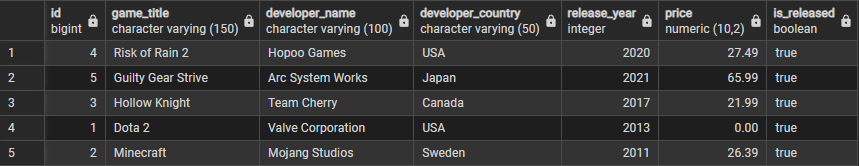
\includegraphics[width=10cm]{view1.png}
		\caption{Результат выборки из представления game\_info\_v}
	\end{figure}
	
	Результат выборки из представления \texttt{game\_genres\_v} (игры с их жанрами) представлен на рисунке~2.
	
	\begin{figure}[H]
		\centering
		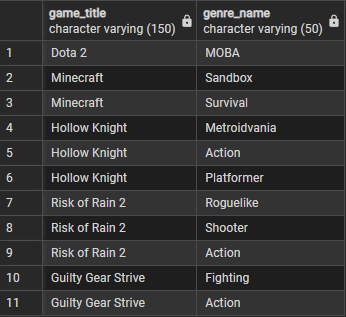
\includegraphics[width=10cm]{view2.png}
		\caption{Результат выборки из представления game\_genres\_v}
	\end{figure}
	
	Результат выборки из представления \texttt{game\_reviews\_v} (отзывы с информацией об играх) представлен на рисунке~3.
	
	\begin{figure}[H]
		\centering
		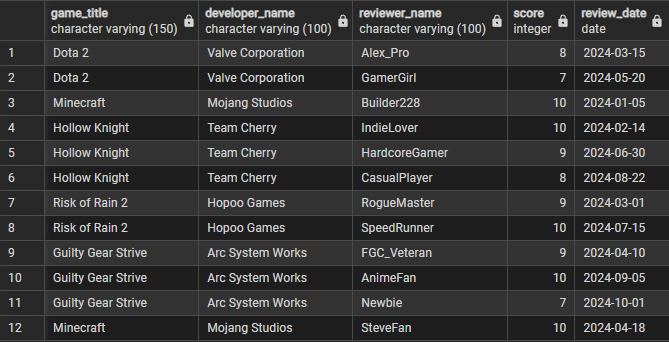
\includegraphics[width=10cm]{view3.png}
		\caption{Результат выборки из представления game\_reviews\_v}
	\end{figure}
	
	Результат выборки из представления \texttt{game\_avg\_rating\_v} (средняя оценка для каждой игры) представлен на рисунке~4.
	
	\begin{figure}[H]
		\centering
		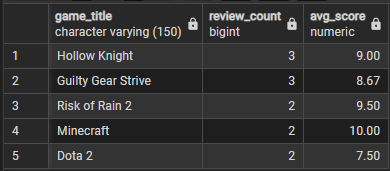
\includegraphics[width=10cm]{view4.png}
		\caption{Результат выборки из представления game\_avg\_rating\_v}
	\end{figure}
	
	\newpage
	
	\section*{Выводы} В ходе выполнения лабораторной работы были освоены основные варианты DML-запросов в PostgreSQL. Создан и выполнен SQL-скрипт заполнения таблиц данными с использованием PL/pgSQL-блока и конструкции RETURNING INTO для поддержания ссылочной целостности. Освоены команды UPDATE и DELETE для изменения и удаления существующих строк. Изучены различные варианты команды SELECT с предложениями WHERE, ORDER BY, LIMIT, OFFSET, а также различными типами соединений (INNER JOIN, LEFT JOIN, CROSS JOIN) и операциями над выборками (UNION, INTERSECT, EXCEPT). Созданы четыре представления с использованием JOIN для получения осмысленной информации по сущностям базы данных. Рабочий материал для последующих лабораторных работ успешно подготовлен.
	
\end{document}